\section{Algoritmy plánovania trajektórie}
\label{kap:2}
Algoritmus plánovania trajektórie je matematický postup alebo procedúra, ktorá určuje cestu alebo pohyb medzi počiatočným a koncovým bodom v priestore.
Cieľom algoritmu plánovania trajektórie je nájsť takú trajektóriu, ktorá spĺňa určité kritériá, ako sú bezpečnosť, efektivita, minimálny čas, minimalizácia spotrebovanej energie, alebo minimalizácia vplyvu na okolie. Tieto kritériá môžu byť definované podľa konkrétnej aplikácie a požiadaviek.

V tejto kapitole sa budeme venovať analýze rôznych algoritmov využívaných v oblasti robotiky. Na základe tejto analýzy budeme schopní určiť, ktorý z týchto algoritmov najlepšie vyhovuje našim potrebám a zabezpečí optimálnu kombináciu medzi presnosťou a rýchlosťou výpočtu. Vybraný algoritmus bude slúžiť ako základ pre úspešnú implementáciu a funkčnosť nášho systému pre plánovanie trajektórií.
 
\subsection{RRT}
\label{kap:2.1}

Algoritmus RRT – z anglického Rapidly-exploring Random Tree, by sa dal do slovenčiny preložiť ako rýchlo rastúci náhodný strom. Algoritmus je v oblasti robotiky veľmi rozšírení a obľúbený vďaka svojej schopnosti rýchlo prehľadávať vysoko dimenzionálny konfiguračný priestor, v ktorom zohľadňuje prekážky v priestore ako aj dynamiku telesa. Autorom algoritmu sú James J. Kuffner a Steven M. LaValle \cite{RRT-Kuffner}.

Ide o algoritmus založený na prehľadávaní konfiguračného priestoru $C$ , kde sa v iteráciách vytvárajú náhodné uzly - $q$, ktorých spájaním vznikajú nové potenciálne cesty. Každý uzol $q$ reprezentuje pozíciu a orientáciu telesa v 2D alebo 3D priestore \cite{RRT-Kuffner}. Pri plánovaní trajektórie je generovaný kontinuálny rad uzlov (obr. \ref{OBRAZOK 1.2.1}), ktorý začína v počiatočnom stave $q_{init}$,  a postupne sa rozrastá až dosiahne koncový stav $q_{goal}$.  Generovanie stromu prebieha v iteráciách kedy sa vždy vygeneruje náhodná konfigurácia $q_{rand}$ a nájde sa k nej najbližší uzol patriaci stromu. Od daného uzla je následne vo vzdialenosti v od uzla $q_{nearest}$ vytvorený nový uzol $q_{new}$. Proces rozrastania stromu sa končí v momente ak sa $q_{new}$  nachádza v okolí cieľovej konfigurácie $q_{goal}$, ktoré je definované vzdialenosťou $d$. 

Ak neuvažujeme voľný konfiguračný priestor $C_{free}$ treba v procese generovania taktiež overovať kolíziu s danými prekážkami v priestore - $C_{obs}$. Novo generovaný uzol stromu sa nesmie nachádzať v priestore prekážky - $C_{obs}$, a ani cesta medzi dvoma susednými uzlami nesmie kolidovať s prekážkou. Pokiaľ uzol spĺňa tieto podmienky, je zaradený do štruktúry stromu, v opačnom prípade je vyradený a proces pokračuje ďalej.

\begin{figure}[h]
	\centering
	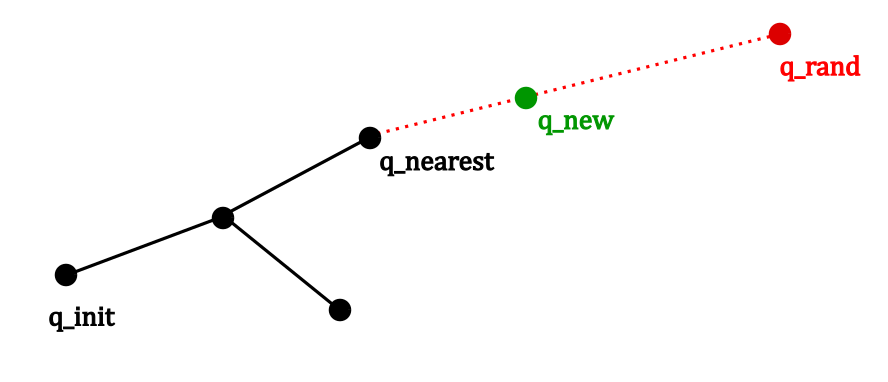
\includegraphics[width=120mm]{img/RRT1.png}
	\caption{Vizualizácia princípu RRT algoritmu }\label{OBRAZOK 2.1} 
\end{figure}    

Algoritmus RRT môže mať nevýhodu v generovaní neoptimálnych výsledkov, pretože generuje body v konfiguračnom priestore náhodne a tvorí trajektóriu ako najkratšiu cestu medzi týmito bodmi. Na zlepšenie výslednej trajektórie existuje niekoľko možností, medzi ktorými je aj RRT*.

\subsection{RRT*}
\label{kap:2.2}

Jedná sa o modifikáciu RRT algoritmu, ktorej cieľom je v porovnaní s pôvodným RRT nájsť kratšiu trajektóriu. Hlavnou úpravou oproti jednoduchému RRT algoritmu je výpočet vzdialenosti z počiatočného do aktuálneho uzlu a následné overenie, či neexistuje v okolí uzol, ktorého vzdialenosť by bola menšia ako vzdialenosť momentálneho prepojenia. Ak táto situácia nastane, algoritmus vyberie prepojenie uzlov , ktoré vytvoria kratšiu trasu. Algoritmy sa tiež líšia ukončovacou podmienkou, kde pre RRT* je určený jasný počet iterácií. Od počtu iterácií závisí výsledný tvar trajektórie, kde so zvyšujúcim sa počtom je algoritmus schopný nájsť kratšie a plynulejšie trasy (obr. \ref{OBRAZOK 1.2.2}).

Tieto úpravy a rozdiely umožňujú algoritmu RRT* dosiahnuť lepšie výsledky v porovnaní s pôvodným RRT, čo ho robí atraktívnou voľbou pre úlohy, kde je kritické dosiahnutie čo najlepšej trajektórie v danom priestore. Je dôležité zohľadniť aj možnosť zvýšenia času výpočtu pri použití algoritmu RRT*. Aj keď má RRT* potenciál nájsť kratšie a plynulejšie trasy ako klasický RRT, zvyšuje sa časová náročnosť algoritmu vzhľadom na výpočet vzdialeností a optimalizácie spojení medzi uzlami.

Pri navrhovaní algoritmu pre plánovanie trajektórií je preto dôležité hľadať rovnováhu medzi kvalitou výsledných trajektórií a časovou náročnosťou výpočtu. Niekedy môže byť akceptovateľné mať mierne suboptimálnu trajektóriu, ak to znamená výrazné zrýchlenie výpočtu. 

\begin{figure}[h]
	\centering
	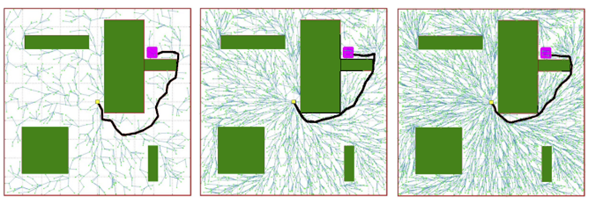
\includegraphics[width=160mm]{img/RRT2.png}
	\caption{Vplyv počtu iterácií na výslednú trajektóriu \cite{RRT-Kuffner}}\label{OBRAZOK 1.2.2} 
\end{figure} 

\subsection{RRT - connect}
\label{kap:2.3}
Algoritmus RRT Connect (spojenie) je ďalšou modifikáciou algoritmu RRT. V procese rozširovania stromovej štruktúry vytvára dva stromy z počiatočnej a koncovej konfigurácie, ktoré sa šíria v konfiguračnom priestore, až kým nedôjde k ich spojeniu a vytvoreniu cesty. (obr. \ref{OBRAZOK 1.2.3}). 

\begin{figure}[h!]
	\centering
	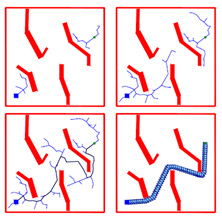
\includegraphics[width=70mm]{img/RRT-connect.png}
	\caption{Prepojenie 2 stromov \cite{RRT-Kuffner}}\label{OBRAZOK 1.2.3} 
\end{figure} 

Tento algoritmus má výhodu v tom, že nájdenie trajektórie je často ľahšie dosiahnuteľné jedným z dvoch možných smerov pohybu medzi dvoma bodmi, čo závisí od prekážok v priestore $C_{obs}$. Použitím algoritmu RRT Connect sa zvyšuje pravdepodobnosť úspešného nájdenia trajektórie od počiatočného bodu ku koncovému.

Tento prístup umožňuje efektívnejšie prehľadávanie konfiguračného priestoru, pretože vytvára dva stromy, ktoré sa šíria smerom k cieľu. Tým sa zvyšuje šanca na rýchlejšie nájdenie vhodnej trajektórie, najmä v prípade, že existuje jasný smer pohybu medzi počiatočným a koncovým bodom.



\subsection{Potenciálové pole}
\label{kap:2.4}

Plánovanie trajektórie na základe potenciálového poľa využíva koncept odpudivých a príťažlivých polí. Príťažlivé pole generuje veľmi nízke hodnoty so stredom v cieľovom bode, ktoré sa so zväčšujúcou sa vzdialenosťou od cieľa zvyšujú. Odpudivé pole naopak generuje veľmi vysoké hodnoty v okolí prekážok v priestore. Kombináciou týchto dvoch polí dostávame tzv. potenciálové pole(obr. \ref{OBRAZOK 1.2.4}) so silným sklonom ku cieľu, čo umožňuje generovanie trajektórie s tendenciou vyhýbať sa prekážkam.

Tento prístup k plánovaniu trajektórie je intuitívny a efektívny v situáciách, kde je cieľ jasne definovaný a potrebné je vyhnúť sa prekážkam v priestore. Použitie potenciálového poľa môže viesť k vytvoreniu plynulej a bezpečnej trajektórie, ktorá dosahuje cieľový bod s minimálnym rizikom kolízií.

\begin{figure}[h]
	\centering
	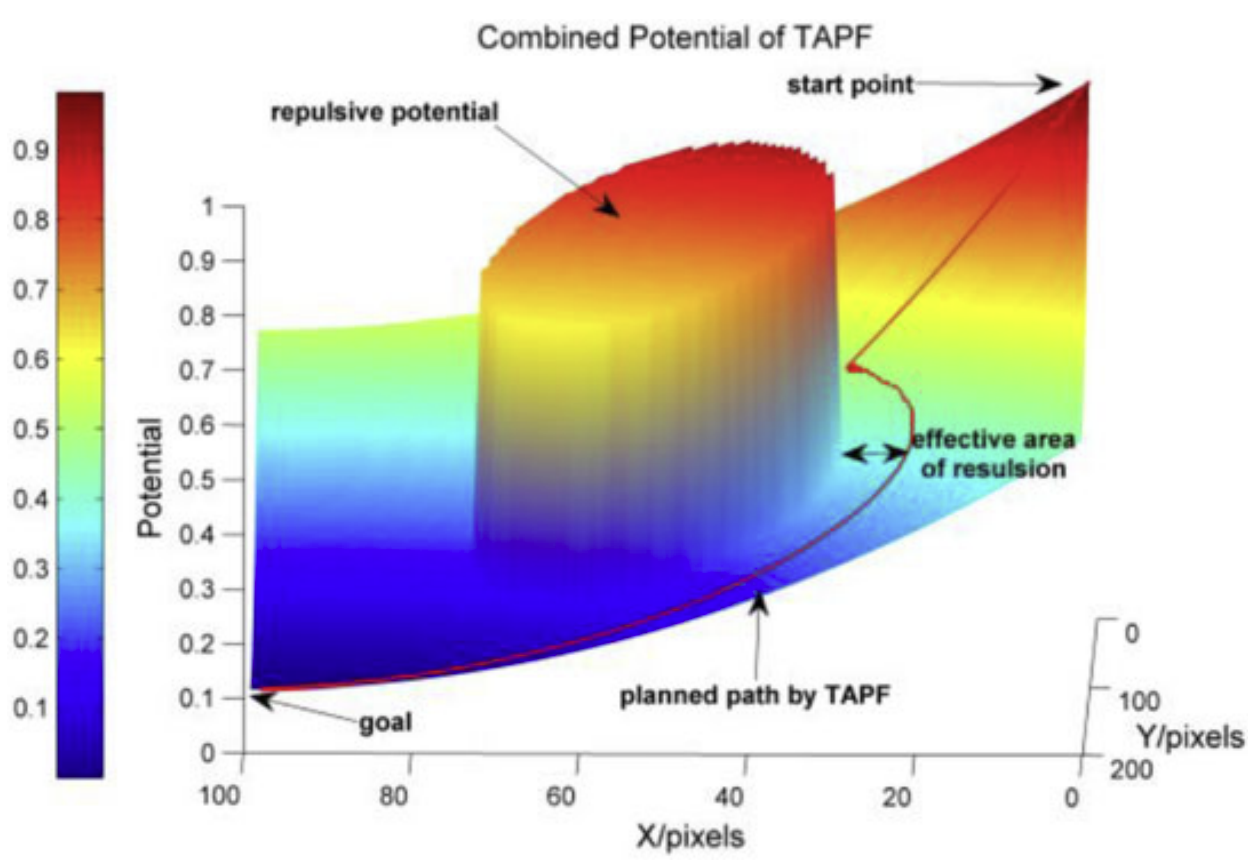
\includegraphics[width=100mm]{img/Potencialove_pole2.png}
	\caption{Potenciálové pole \cite{Potencialove_pole}}\label{OBRAZOK 1.2.4} 
\end{figure} 

\subsection{STOMP algoritmus}
\label{kap:2.5}

Algoritmus STOMP (Stochastic Trajectory Optimized Motion Planner) funguje na základe iteratívneho procesu, ktorý sa skladá z niekoľkých krokov. Počiatočná trajektória je generovaná ako lineárna interpolácia medzi počiatočným a koncovým bodom. STOMP pracuje s fixným počtom krokov na trajektóriu, nazývaných "timesteps", a tiež s definovaným počtom iterácií, v ktorých algoritmus hľadá trajektóriu. Následne je generovaný šum, ktorý je aplikovaný na každý bod trajektórie, čo umožňuje prehľadávanie konfiguračného priestoru v okolí počiatočnej trajektórie(obr. \ref{OBRAZOK 1.2.5}).

Každá vygenerovaná trajektória je potom ohodnotená pomocou účelovej funkcie. V prípade, že priestor obsahuje veľké množstvo prekážok, môže nastať situácia, kedy algoritmus nenájde riešenie. Zvýšením hodnoty šumu sa zväčší priestor prehľadávania a zvýši sa pravdepodobnosť nájdenia bezkolíznej trasy, avšak za cenu zníženej optimalizácie trajektórie. Toto môže byť riešené zvýšením počtu iterácií, avšak to môže mať za následok zvýšenie výpočtového času algoritmu.

Zvolenie správnych parametrov a vyváženie medzi priestorom prehľadávania, optimalizáciou trajektórie a výpočtovým časom je kľúčové pre úspešné použitie algoritmu STOMP v plánovaní trajektórie v prostredí s prekážkami.

\begin{figure}[h]
	\centering
	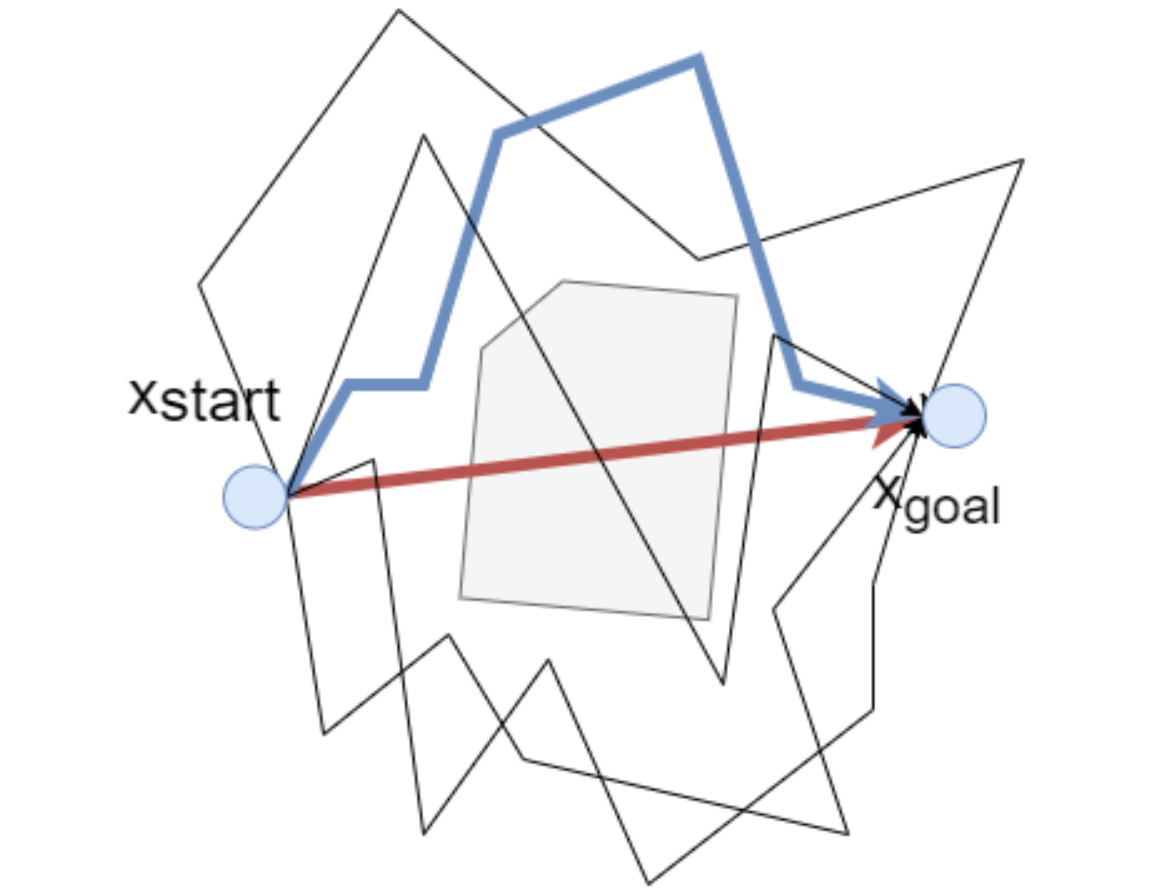
\includegraphics[width=100mm]{img/STOMP.png}
	\caption{Generované trajektórie \cite{STOMP}}\label{OBRAZOK 1.2.5} 
\end{figure} 

\begin{figure}[h]
\end{figure} 


